\documentclass{article}
\usepackage{graphicx}
\usepackage{hyperref}
\usepackage{url}
\usepackage{listings}

\setlength{\parskip}{1em}

\begin{document}


\title{Scripting ICE with EASE}

In addition to interacting with tools via the ICE user interface, ICE also
provides a scripting framework based on the Eclipse Advanced Scripting
Environment (EASE). 

\section{Installation and Configuration}

Although EASE is pre-installed in the ICE application, there are a few
additional components that need to be installed in order to provide a Python
scripting engine.

\subsection{EASE Jython Installation} 

The first step is to install the EASE Jython engine. This can be done via the
official EASE
repository\footnote{\texttt{https://dl.bintray.com/pontesegger/ease-jython}}
using the Eclipse Update Manager, but is more simply achieved using the Install EASE Components menu.

To installed the Jython engine, select \texttt{Help $\rightarrow$ Install
EASE Components} from the ICE menu bar. Check the box next to the EASE Jython
Integration entry and click Finish. Follow the prompts to install the component,
and restart Eclipse when asked.

\begin{center}
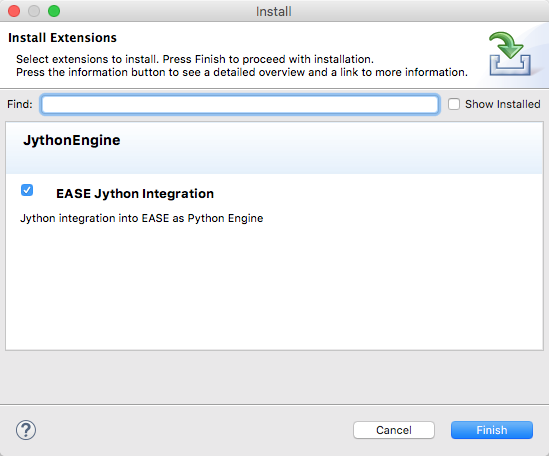
\includegraphics[width=10cm]{images/ease-marketplace}
\end{center}

\subsection{PyDev Installation (optional)} 

It is possible to edit Python scripts in Eclipse using the default text editor,
however it is much more productive to use the PyDev Eclipse development
environment. In addition to the usual syntax coloring and other advanced editing
features you'd expect in Eclipse, PyDev also provides the ability to run and
debug Python programs from within the Eclipse environment.

PyDev can be easily installed from using the Eclipse Marketplace client as
follows. From the ICE menu bar, select \texttt{Help $\rightarrow$ Eclipse
Marketplace\ldots}, type ``pydev'' in the Find field, then click the \texttt{Go}
button.
After a few seconds, you should see an entry for PyDev. Simply click the
\texttt{Install} button and follow the prompts to install the feature. Once
Eclipse has been restarted, any Python scripts ending in ``.py'' will be recognized by
PyDev and opened in the Python editor by default.

\begin{center}
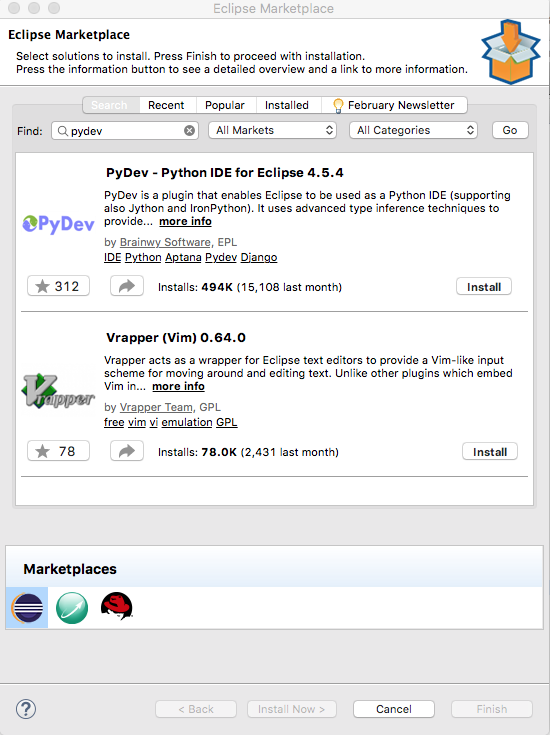
\includegraphics[width=10cm]{images/pydev-marketplace}
\end{center}

\subsection{EASE Configuration}

By default, EASE is configured to use the javascript (Rhino) engine. Since this
tutorial assumes that the preferred environment is Python, we recommend changing
this default. This is done through the Scripting preferences.

To set the script engine default, select \texttt{Window $\rightarrow$
Preferences\ldots} in the ICE menu bar. (On Mac OS X, Preferences\ldots is
instead located under Eclipse ICE in the menu bar.) Open the \texttt{Scripting}
tree item on the left side of the preferences window, then select
\texttt{Shell}. Finally, select \texttt{Python (Jython)} from the
\texttt{Preferred Engine:} dropdown, then click on \texttt{OK}.

\begin{center}
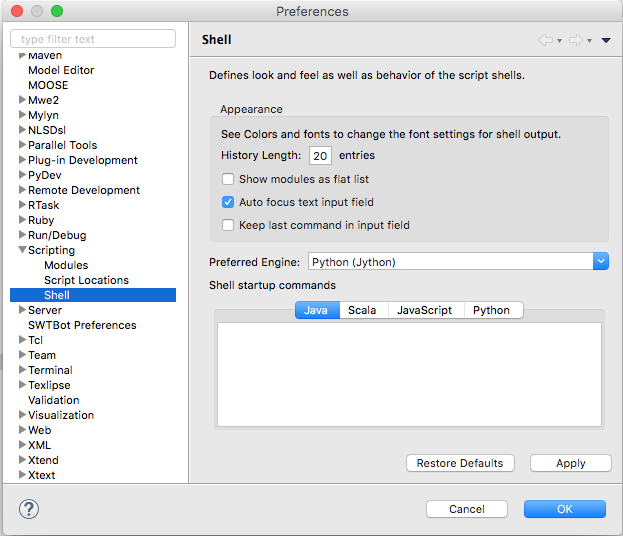
\includegraphics[width=10cm]{images/scripting-prefs}
\end{center}


\section{Creating and Running Scripts}

There is nothing special about creating and running EASE scripts. They can be
created in a variety of ways using the development tools available in ICE, and
then run later when needed. For this tutorial, we will be creating the scripts
using PyDev (or any text editor) and running them directly using the \texttt{Run As
$\rightarrow$ EASE Script} context menu.

EASE also provides a perspective for creating, managing, debugging, and running
scripts called the \texttt{Scripting} perspective. This perspective contains
views for running script commands interactively, and for exploring script modules.
For additional information on the
\texttt{Scripting} perspective and other EASE features, see the EASE
documentation\footnote{\path{http://eclipse.org/ease/documentation}}.

\subsection{Creating a Python Script}

The easiest way to create a Python script is to simply create a text file ending
in ``.py'' in an existing project. If your scripts will be used with stand-alone Python
programs, you can use PyDev to create a Python project, but in general, any kind
of project will suffice.

First, let's create a project to hold the scripts. To do this, right click
anywhere in the \texttt{Project Explorer} view and select \texttt{New
$\rightarrow$ Project\ldots} or click on the \texttt{New} button in the toolbar. Once you do
this, you should see the \texttt{Select a wizard} dialog like the one shown below.

\begin{center}
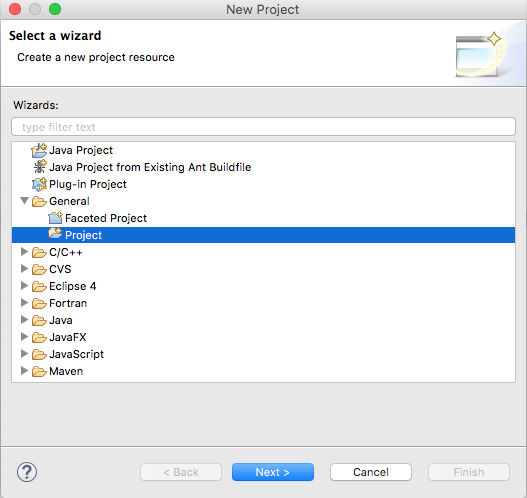
\includegraphics[width=10cm]{images/newproject}
\end{center}

Open the \texttt{General} folder in the list of wizards, and select the \texttt{Project}
wizard as shown. Then click on the \texttt{Next \textgreater} button which
should open the \texttt{New Project} wizard. This is shown below.

\begin{center}
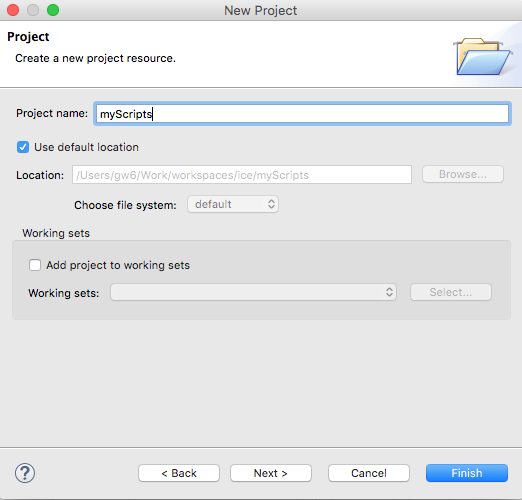
\includegraphics[width=10cm]{images/newproject_wiz}
\end{center}

Enter a name for the project in the \texttt{Project name:} field and then click the
\texttt{Finish} button. You can leave all the other options set to their default
values.

You should now see a folder with the name you specified appear in the
\texttt{Project Explorer} view. You can now create a Python file in this folder by
right clicking on the folder and selecting \texttt{New $\rightarrow$ File} from
the context menu. This will display the \texttt{New File} dialog as shown below.

\begin{center}
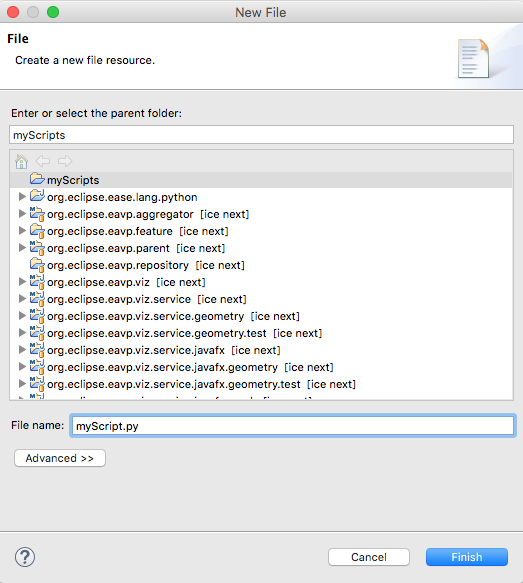
\includegraphics[width=10cm]{images/newfile}
\end{center}

At this point all that remains to be done is enter the name of the file in the
\texttt{File name:} field and click on the \texttt{Finish} button. This will
create the file and automatically open the PyDev editor (assuming you installed
PyDev).

\subsection{Writing a Python Script}

EASE hides many of the details that would normally be required to manipulate
Java objects and perform actions in the Eclipse IDE. It does this by
encapsulating typical actions into simple script commands that can be easily
invoked from scripts that you write. These commands are collected together into
``modules''. You can see which modules are available, and the commands that they
contain, using the \texttt{Modules Explorer} view. This view can be opened by
selecting \texttt{Window $\rightarrow$ Show View $\rightarrow$ Other\ldots} to
open the \texttt{Show View} dialog, as shown below.

\begin{center}
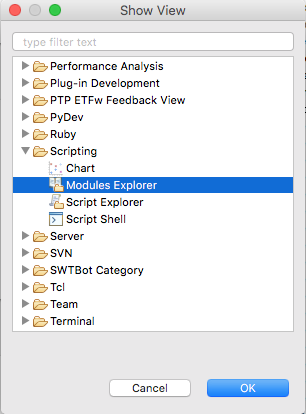
\includegraphics[width=6cm]{images/showview}
\end{center}

Form this dialog, open the \texttt{Scripting} folder and select the
\texttt{Modules Explorer}, then click on \texttt{OK}. This will open the
\texttt{Modules Explorer} view which can be used to explore the modules and commands
that are available for use in EASE scripts.

\begin{center}
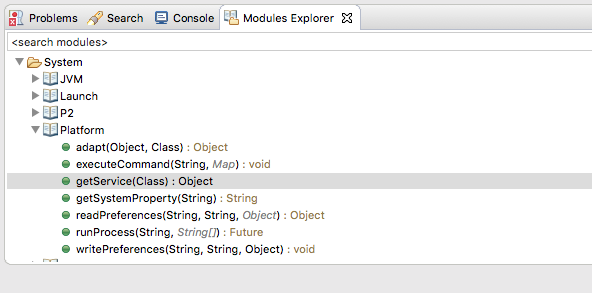
\includegraphics[width=10cm]{images/modulesexplorer}
\end{center}

For the purposes of this tutorial, we will just be using the
\texttt{Platform} module. In order to load a module, we use the
\texttt{loadModule()} function in Python. The argument to this function is a
string representation of the module path, which in this case will be
\texttt{/System/Platform}. 

Enter the following command as the first line of the script file:

\lstset{basicstyle=\ttfamily\small, breaklines}

\begin{lstlisting}[frame=single,language=Python]
loadModule("/System/Platform")
\end{lstlisting}

Once this module has been loaded, a number of additional functions become
available. We want to obtain a reference to the core ICE service, which is used
as the starting point for manipulating ICE models. This is done by adding the
following line:

\begin{lstlisting}[frame=single,language=Python]
coreService = getService(org.eclipse.ice.core.iCore.ICore)
\end{lstlisting}

Once a reference to the core services has been obtained, we can use this to
obtain a reference to the Reflectivity Model. This is done by adding the
following line:

\begin{lstlisting}[frame=single,language=Python]
reflectModel = coreService.getItem(int(coreService.createItem("Reflectivity Model")))
\end{lstlisting}

Note that the \texttt{createItem()} method will return a string representing the
number of that item, so \texttt{int()} is used to convert it to an integer, which is the
argument expected by \texttt{getItem()}.

In this example, we're just going to accept the default inputs for the model, so
the only thing left to do it process the model. This is done using the core
service \texttt{processItem()} as follows:

\begin{lstlisting}[frame=single,language=Python]
res = coreService.processItem(reflectModel.getId(), "Calculate Reflectivity", 1)
\end{lstlisting}

Finally, let's print out the result of processing the model to see if it was
successful.

\begin{lstlisting}[frame=single,language=Python]
print "result was: %s" % res
\end{lstlisting}

\subsection{Running a Python Script}

Once you have created Python script, is can be easily launched using the Run As
context menu. Simply right-click on the Python file, then select \texttt{Run As
$\rightarrow$ EASE Script}. EASE will automatically recognize the file type and
run the script with the appropriate engine. Any (textual) output generated by
the script will be displayed in the Console view shown below\footnote{
In this case the \texttt{processItem()} function returns \texttt{InfoError}
because it hasn't been correctly configured before the model was processed. We
will see how to fix this later in the tutorial.}.

\begin{center}
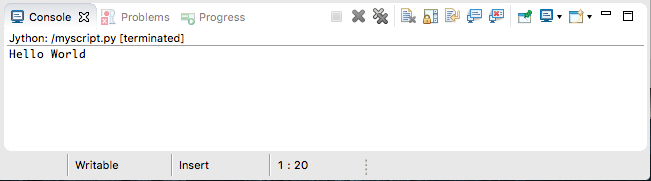
\includegraphics[width=12cm]{images/console}
\end{center}

Re-running the script is simple as ICE has automatically added the most recently
executed run configuration to the run button. Just click on the

\includegraphics[width=0.5cm]{images/runbutton} icon to re-run the last script.
You can also click on the small triangle next to the button to see a list of 
recent launches and re-run them if desired. 

\section{Using the Sample Scripts}

\lstset{basicstyle=\ttfamily\scriptsize, breaklines}
\makeatletter
\def\lst@lettertrue{\let\lst@ifletter\iffalse}
\makeatother

We have provided a number of sample scripts to show how ICE can be
scripted using EASE.
These scripts are located in the
\path{org.eclipse.ice.examples.reflectivity} package that is already loaded
in your workspace. The scripts can also be obtained by cloning the ICE Git
repository\footnote{\texttt{http://github.com/eclipse/ice.git}},
then manually importing the \path{org.eclipse.ice.examples.reflectivity}
package.

There are four sample scripts that demonstrate how a reflectivity model
can be created, configured and executed. The scripts are described in
more detail in the following sections.

\subsection{createAndProcessPython.py} 

This is a simple script
that demonstrates how to create a reflectivity model and process the model to
obtain a result. The default model inputs are used for the computation.

\lstinputlisting[frame=single,language=Python]{samples/createAndProcessPython.py}

\subsection{createAndEditPython.py} 

This script extends the
\texttt{createAndProcessPython.py} script by editing the input to the model
programmatically. The model is then processed to obtain the results.

\lstinputlisting[frame=single,language=Python]{samples/createAndEditPython.py}

\subsection{iterateChangeParameterPython.py} 
This script demonstrates how to create
multiple reflectivity models with varying input parameters. The models are created
and processed sequentially.

\lstinputlisting[frame=single,language=Python]{samples/iterateChangeParameterPython.py}

\subsection{listFromScratchPython.py} 
This script demonstrates how to create a
reflectivity model and programmably create and set up the layers in the model.
The model is then process to obtain the results.

\lstinputlisting[frame=single,language=Python]{samples/listFromScratchPython.py}

\end{document}
